\begin{table}[ht]
    \centering
    \caption{\label{tab:energy_densities}Spezifische Energie und Energiedichte für eine representative \ce{LiCoO2} (LCO) Kathode und eine Grafitanode in verscheidenen Referenzsystemen.\cite{Son2021}}
    \begin{tabular}[t]{lccccc}
    \toprule
    \multirow{2}{*}{}
    &\multirow{1}{*}{Materialebene} % \textsuperscript{*}
    &\multirow{1}{*}{Elektrodenebene}
    &\multicolumn{2}{c}{Zellebene}
    \\ \cmidrule{2-5}
    &\makecell{Aktivmaterial\\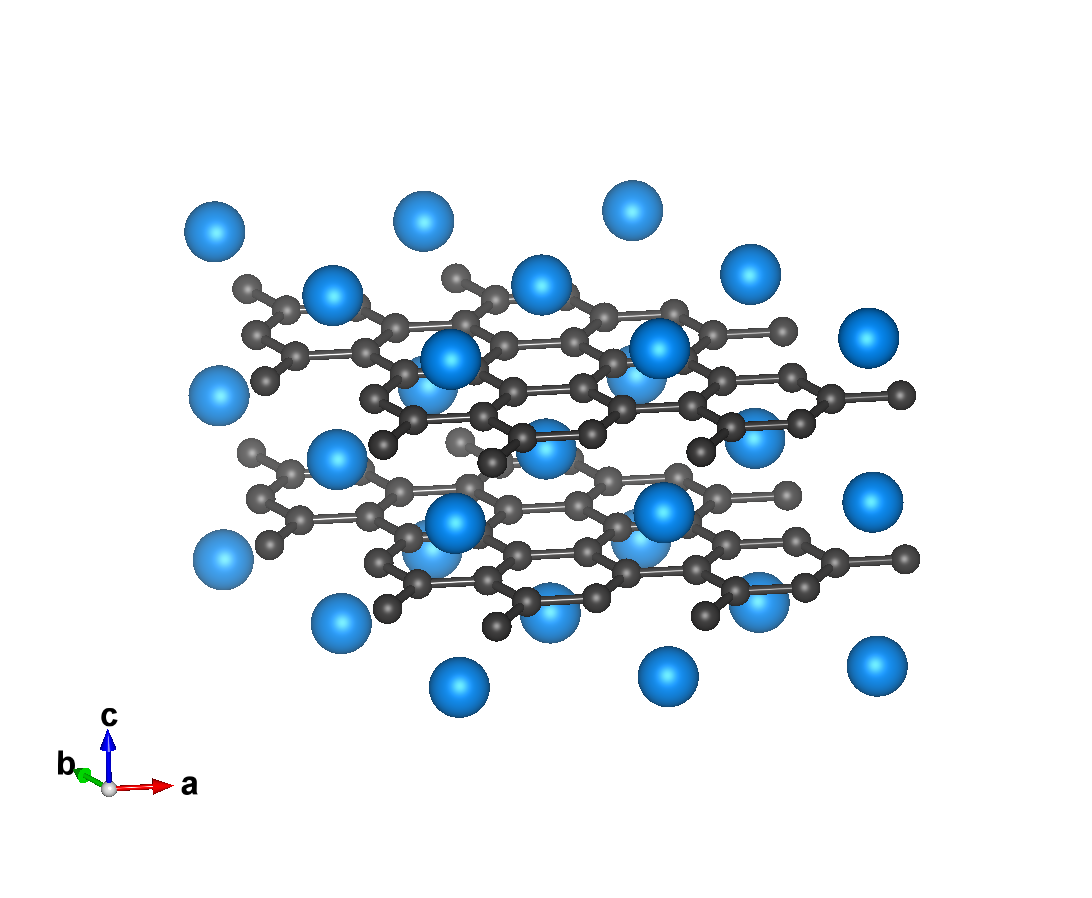
\includegraphics[width=0.125\textwidth]{CathodeMaterials/LiC6.png}\vspace{-1em}}
    &\makecell{Elektrode\\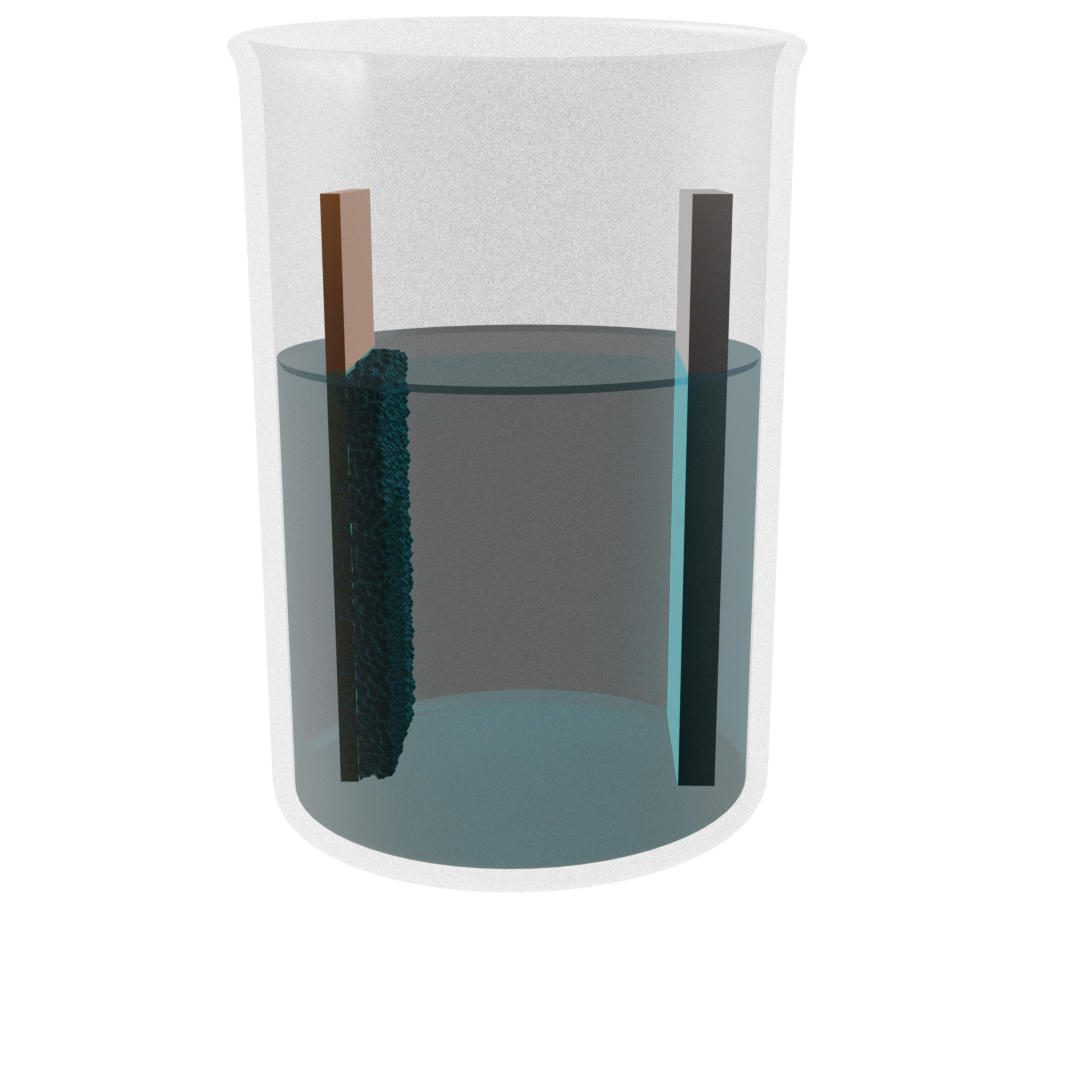
\includegraphics[width=0.1\textwidth]{EnergyDensitiesScales/Electrode.png}\vspace{-1em}}
    &\makecell{Knopfzelle\\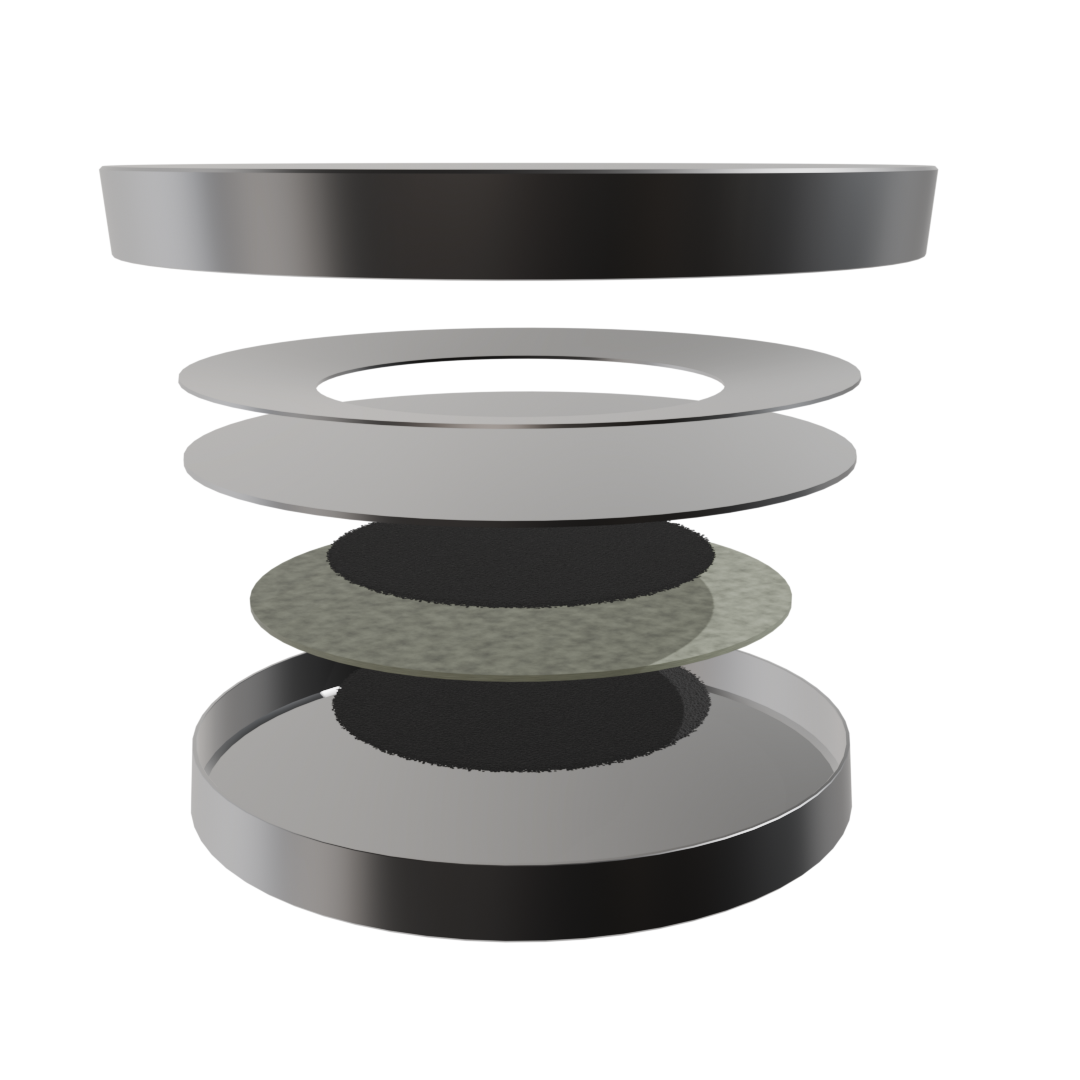
\includegraphics[width=0.1\textwidth]{EnergyDensitiesScales/CoinCell.png}\vspace{-1em}}
    &\makecell{Pouchzelle\\(1 Ah)\\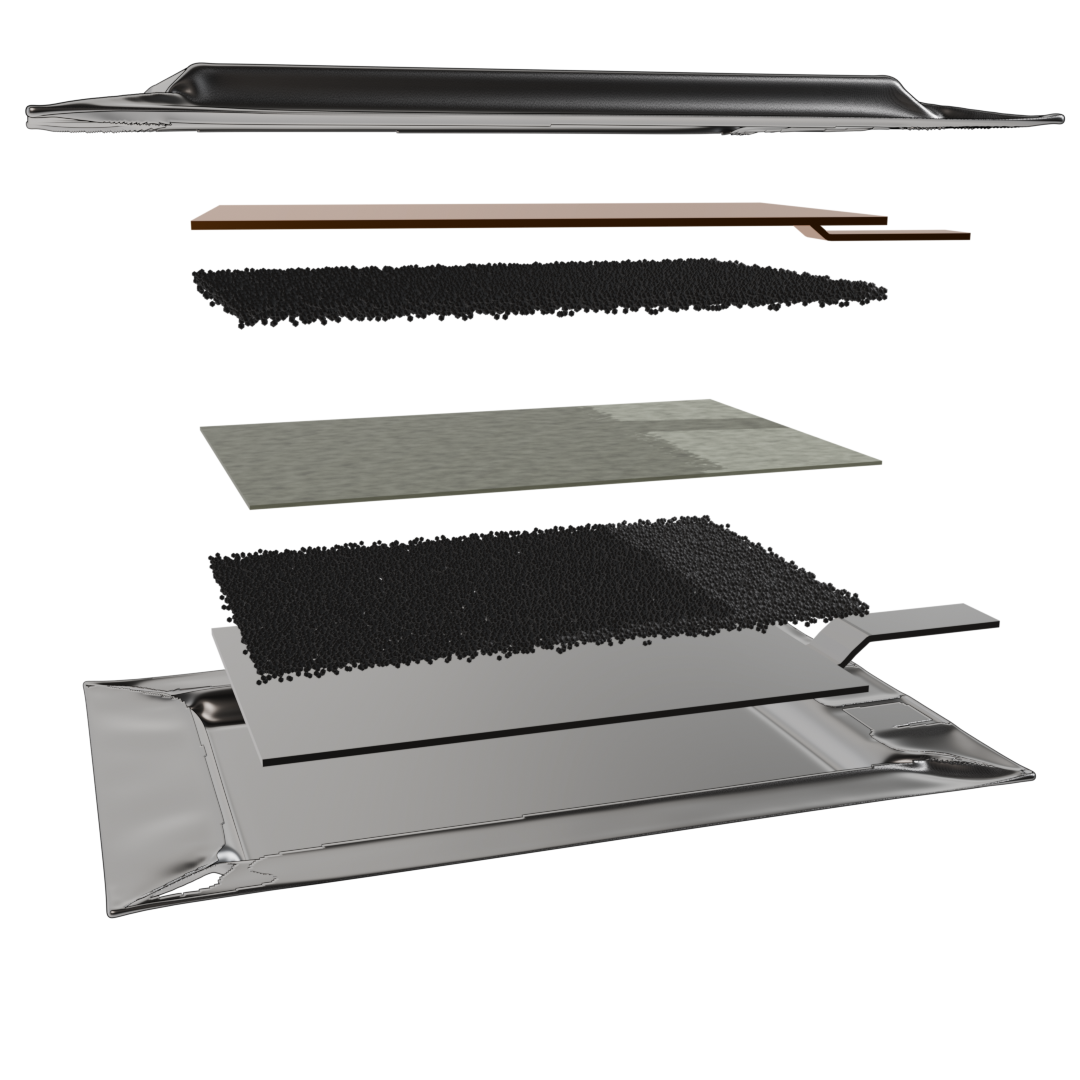
\includegraphics[width=0.1\textwidth]{EnergyDensitiesScales/PouchCell.png}\vspace{-1em}}
    \\
    \midrule
    \makecell{Spezifische Energie\\ $\left[ \si{\watt \hour \per \kg} \right]$} & 627 & 514 & 5 & 260\\
    \makecell{Energiedichte\\ $\left[ \si{\watt \hour \per \liter} \right]$} & 3166 & 1527 & 19 & 414\\
    \bottomrule
    \end{tabular}
    %\noindent{\footnotesize{\textsuperscript{*} Die Abkürzung nicht auffindbar (n.a.) wurde benutzt.}}
\end{table}%